%%%%%%%%%%%%%%%%%%%%%%%%%%%%%%%%%%%%%%%%%
% Peking Univ. Physical Review (cn)
%
% LaTeX Template
% Version 2.1
% Release 03/19/18
%
% Original author:
% Mathias Legrand (legrand.mathias@gmail.com)
%
%%%%%%%%%%%%%%%%%%%%%%%%%%%%%%%%%%%%%%%%%
%
%----------------------------------------------------------------------------------------
%	PACKAGES AND OTHER DOCUMENT CONFIGURATIONS
%----------------------------------------------------------------------------------------
\RequirePackage{times}      % Loads the Times-Roman Fonts
%\RequirePackage{mathptmx}   % Loads the Times-Roman Math Fonts
\documentclass[10pt,a4paper,twocolumn]{PPRAcn} % Document font size

\usepackage[UTF8]{ctex}
\usepackage{listings}
\lstset{language=matlab, escapeinside=``, breaklines=true, backgroundcolor=\color{lightgray!40!white}, frame=none,extendedchars=false, keywordstyle=\color{blue!70}\bfseries, basicstyle=\ttfamily,
commentstyle=\ttfamily\color{green!40!black}, showstringspaces=false}
\usepackage[english]{babel} % Specify a different language here - english by default
\usepackage{lipsum} % Required to insert dummy text. To be removed otherwise
\usepackage{bm,caption,textcomp,subfigure,float}
\usepackage[keeplastbox]{flushend}
\usepackage{lastpage}
\usepackage{geometry}
\newgeometry{top=28mm,bottom=25mm,left=20mm,right=25mm}

\newcommand{\upcite}[1]{\textsuperscript{\textsuperscript{\cite{#1}}}}

%----------------------------------------------------------------------------------------
%	COLUMNS
%----------------------------------------------------------------------------------------

\setlength{\columnsep}{7.0mm} % Distance between the two columns of text
\setlength{\fboxrule}{0.75pt} % Width of the border around the abstract
\setlength{\abovecaptionskip}{5pt}
\setlength{\belowcaptionskip}{0pt}

%----------------------------------------------------------------------------------------
%	COLORS
%----------------------------------------------------------------------------------------

\definecolor{color1}{RGB}{0,0,90} % Color of the article title and sections
\definecolor{color2}{RGB}{0,20,20} % Color of the boxes behind the abstract and headings

%----------------------------------------------------------------------------------------
%	HYPERLINKS
%----------------------------------------------------------------------------------------

\usepackage{hyperref} % Required for hyperlinks
\hypersetup{hidelinks,colorlinks,breaklinks=true,urlcolor=color2,citecolor=color1,linkcolor=color1,bookmarksopen=false,pdftitle={Title},pdfauthor={Author}}

%----------------------------------------------------------------------------------------
%	ARTICLE INFORMATION
%----------------------------------------------------------------------------------------

\newcommand{\keywordname}{Keywords} % Defines the keywords heading name
\captionsetup[figure]{name={图}}
\captionsetup[table]{name={表}}
\captionsetup{font={small}}
%\JournalInfo{Journal, Vol. XXI, No. 1, 1-5, 2013} % Journal information
%\Archive{Additional note} % Additional notes (e.g. copyright, DOI, review/research article)

\PaperTitle{从多等价Dirac锥体系到高Chern数量子反常霍尔效应:自旋轨道耦合和磁诱导下的石墨烯} % Article title
\Authors{JLZhang1996\textsuperscript{1*}} % Authors
\affiliation{

	\quad
	\textsuperscript{1} {GDPi}
	\qquad
	*:jlzhang1996@gmail.com
} % Author affiliation

\Abstract{
	\phantom{田田}石墨烯是非常典型的二维Dirac材料,由于良好的调控性质,在近些年被广泛关注。根据现有的能带反转(Band Inversion)的图像,本文研究了Rashba自旋轨道耦合效应和磁Zeeman场下,多Dirac锥材料实现高Chern数量子霍尔效应的可能性。由于石墨烯具有位于$\mathbf{K}$和$\mathbf{K'}$两个等价Dirac锥,该体系出现了$C=2$的量子反常霍尔效应。并且,利用求解迭代格林函数和开边界的格点哈密顿量,表明了局域在Zigzag边界处分别存在两条手性边缘态,最后讨论了这一特殊的边缘态在输运实验上的奇特性质。
}


\Keywords{\phantom{田田}多Dirac锥体系,石墨烯,高Chern量子反常霍尔效应}
% 如不需要关键词可直接删去花括号中内容

 %这是标题,作者和摘要(关键词)

%----------------------------------------------------------------------------------------

\begin{document}

\flushbottom % Makes all text pages the same height

\maketitle % Print the title and abstract box
%\tableofcontents % Print the contents section

\thispagestyle{empty} % Removes page numbering from the first page

%----------------------------------------------------------------------------------------
%	ARTICLE CONTENTS
%----------------------------------------------------------------------------------------

	\section{引言}\label{sec:intro}
    石墨烯是一种二维碳纳米材料,具有蜂窝状的六角晶型,如图\ref{fig:graphene}~(a)所示。石墨烯的外层电子共有四个,其中三个发生sp2杂化,与周围碳原子之间形成$\sigma$键,非常稳固;另一个电子处于垂直方向上的$p_z$轨道,形成离域的大$\Pi$键,作用较弱。正是由于$\Pi$电子作用力很弱,游离在整个晶面中,因此给石墨烯带来了超高的电导率。而在石墨的多层结构中,层间是由范德瓦尔兹力连接,因而层与层之间很容易剥离。sp2形式杂化的碳原子六角密排而成的二维蜂窝状晶体结构,其碳-碳键长约0.142nm,单层厚度0.334nm,仅为头发丝直径的20万分之一,是目前发现的最薄的层状材料。
    \begin{figure}
      \centering
      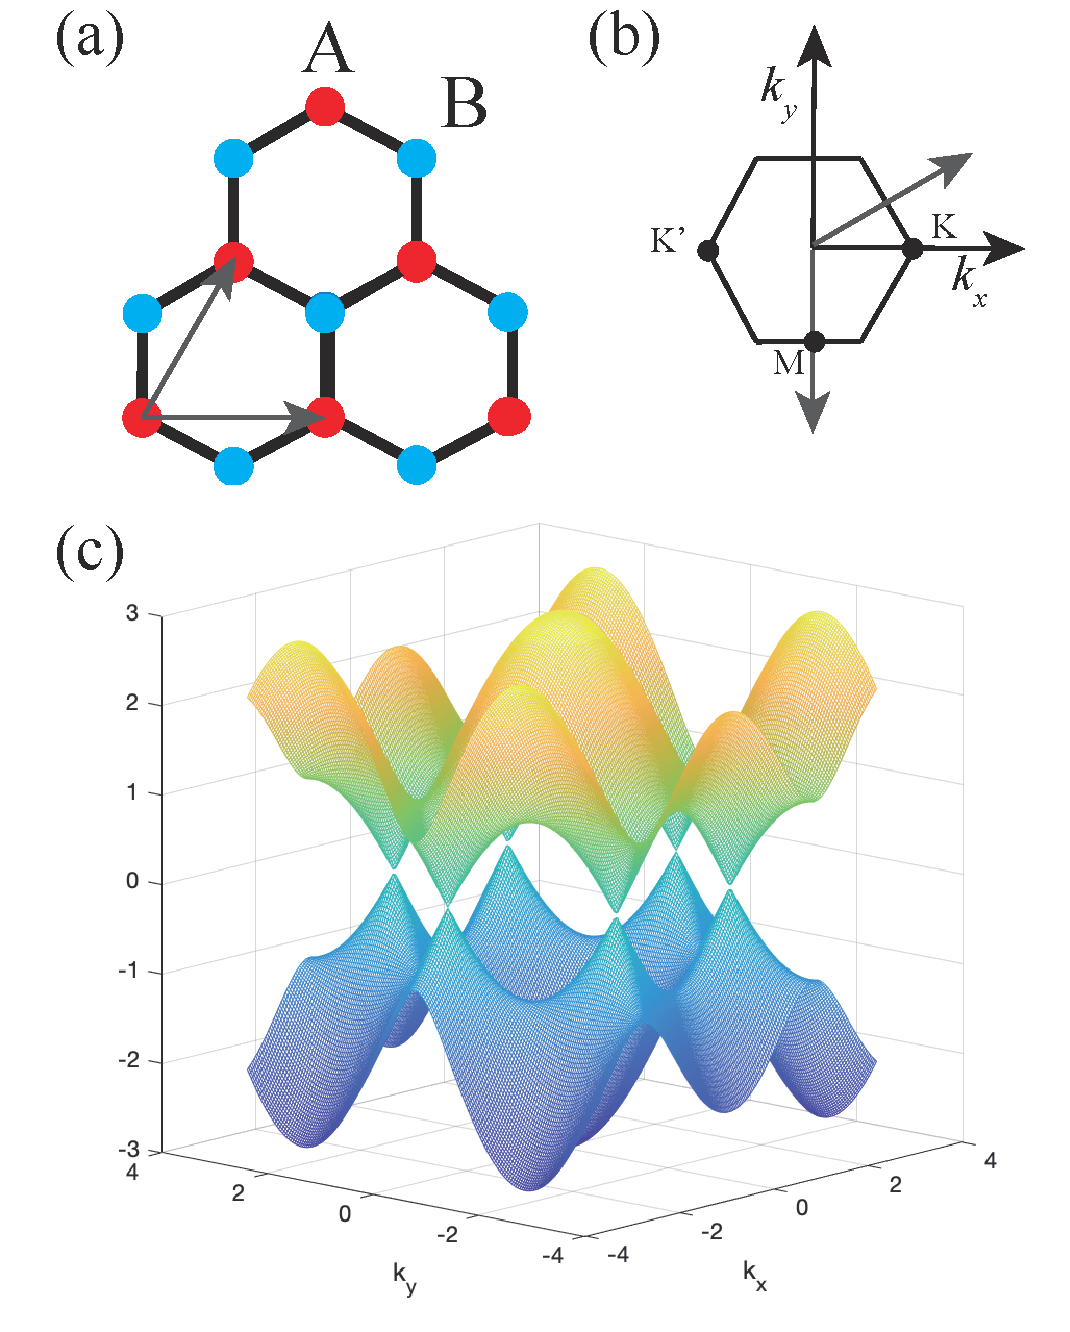
\includegraphics[width=0.5\textwidth]{pic/fig0.pdf}
      \caption{(a)石墨烯晶格;(b)石墨烯第一布里渊区;(c)第一布里渊区能带。}\label{fig:graphene}
    \end{figure}
    2004年英国曼彻斯特大学的Geim教授课题组首次在实验中巧妙的用机械剥离的办法得到单层石墨烯,此后诸多的实验揭示了石墨烯与众不同的物性\cite{novoselov2005two,novoselov2007rise,Castro2009},包括力学、热学上的稳定性等等。此外,石墨烯的导电性为目前已知的二维材料中导电性能最为出色的。
	
    石墨烯的能带结构非常特殊,在布里渊区边界的$\mathbf{K}$点及$\mathbf{K}'$点处,如图\ref{fig:graphene}~(b)所示,由于偶然简并,导带与价带接触于一点,且具有线性的色散关系, 如图\ref{fig:graphene} (c)所示。这种结构被称为Dirac锥,这个锥是由质量为零的Dirac方程描述的,所以这个锥被称为Dirac锥,而交点叫做Dirac点,它的行为表现为无质量的Dirac费米子。因此电子在石墨烯内传输时不易因阻力而发生散射,故石墨烯中的电子迁移率异常之高。研究表明,石墨烯中的电子迁移率高达$2\times 10^6 $cm$^2$/V$\cdot$ s,约为硅电子迁移率的140倍\cite{Castro2009,Kane2005,Kane2005_1}。

    二维拓扑绝缘体,即具有与普通绝缘体不同拓扑数的体系,首先表现出的现象即为量子自旋霍尔效应(Quantum Spin Hall Effect,QSHE)。在石墨烯中,C.L.Kane和E.J.Mele首先指出,当这个体系存在自旋轨道耦合时,Dirac点处会打开带隙,在特定的参数范围内,会出现自旋极化的一维边缘态,如图所示。也就是说,在其边界上,存在一对导电通道,它们自旋相反且沿相反的方向传输,这样的输运特性叫做螺旋性(helicity),是自旋动量锁定(spin-momentum locking)的。因为每个通道的霍尔电导为$\frac{e^2}{h}$,所以总的霍尔电导为零。而它的自旋霍尔电导则为$\sigma_{xy,\text{SPIN}}=2\frac{e}{4\pi}$。故其为量子自旋霍尔态。量子自旋霍尔态可以看做是两个量子霍尔态的组合,它的螺旋性的边态是两个自旋极化的手性态的组合,这就形成了时间反演保持的配对\cite{Qi2011}。

    \begin{figure}
      \centering
      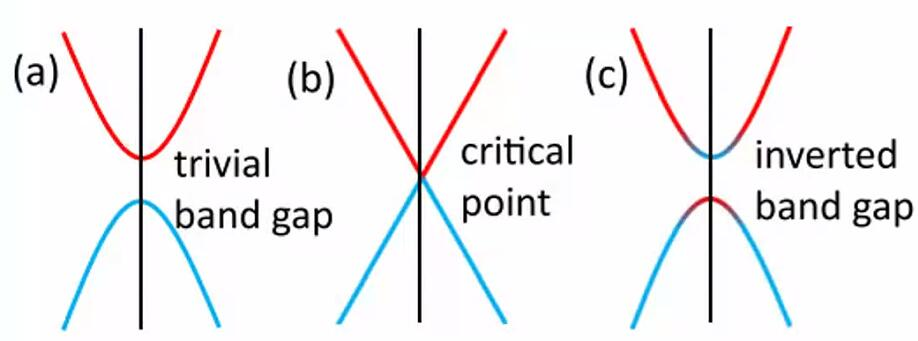
\includegraphics[width=0.5\textwidth]{pic/fig0_2.jpg}
      \caption{能带反转示意图:(a)平庸绝缘态带隙(b)偶然简并在临界点处闭合(c)能带反转并产生非平庸带隙\cite{Bansil2016}}\label{fig:BI}
    \end{figure}

    相较于传统模型中、强磁场形成量子化朗道能级导致了霍尔电导的整数化效应,Haldane\cite{Haldane1988}发现在六角蜂窝状晶格中引入交错磁通破坏时间反演对称性后,在无外场的条件下仍能打开一个拓扑非平庸的能隙,实现反常的量子霍尔效应。在有如上晶格结构的石墨烯中,可通过添加Rashba自旋轨道耦合实现磁通的交错,并引入磁交换作用破坏时间反演对称性,最终解出在石墨烯中受拓扑保护的手性边缘态。在实验上,可以在石墨烯晶格中引入吸附磁性原子提供局域磁矩,或增强样品与反铁磁衬底间的耦合作用,以期待实现室温中的量子反常霍尔效应。

    本文主要基于能带反转的图像,介绍如何通过自旋轨道耦合和磁Zeeman效应在石墨烯体系此类多Dirac锥体系实现$C=2$的量子霍尔效应。不同于薄层多带体系中高Chern数的实现\cite{Jiang2012,WangJ2013},该高Chern数来源于石墨烯能带$\mathbf{K}$和$\mathbf{K}'$的等价性。主要行文安排如下:\ref{sec:intro}主要介绍石墨烯及其量子反常霍尔效应的背景和实现量子反常霍尔效应的指导原则,\ref{sec:model}给出了格点模型和描述边缘态的方法,然后,\ref{sec:result}分析边缘态的输运性质,最后,\ref{sec:summary}给出总结。其他一些支持材料列在\ref{sec:code}。

	\section{理论模型及其能带}\label{sec:model}
	首先,石墨烯晶体结构空间群属于P6/mmm(No.191),具有$C_{6v}$的对称性,可以用2D六角晶格模型进行描述,利用重元素掺杂可以增强自旋轨道耦合(SOC)强度\cite{rortais2018},从而实现能带反转,通过磁近邻\cite{Mingda2017}或者磁掺杂\cite{chang2013}等手段可以可以实现对于磁Zeeman效应的调控。利用紧束缚近似,可以写出格点哈密顿量
	\begin{equation}
	\begin{aligned}
		H=&-t\sum_{\langle i,j\rangle\alpha}c_{i,\alpha}^\dagger c_{j,\alpha}\\
            &+i t_{\text{SO}} \sum_{\langle i,j\rangle\alpha\beta}\hat{\mathbf{e}}_z\cdot(\mathbf{\sigma}_{\alpha,\beta}\times\mathbf{d}_{i,j})c_{i,\alpha}^\dagger c_{j,\beta}	\\
		&+\lambda\sum_{i,\alpha} c_{i,\alpha}^\dagger c_{i,\alpha},
		\end{aligned}
	\end{equation}
	其中,$c^\dagger_{i,\alpha}(c_{i,\alpha})$ 是自旋为$ \alpha $的电子在格点$ i $的产生(湮灭)算符,$\mathbf{\sigma}$是自旋-$\frac{1}{2}$的Pauli矩阵,$\langle i,j\rangle$表示最近临格点,$\mathbf{d}_{i,j} $ 是归一化后的$\mathbf{r}_i-\mathbf{r}_j$。第一项为最近临的跃迁项,表示强度为$t$的动能项,第二项描述强度$t_{\textbf{SO}}$的Rashba型的自旋轨道耦合项,第三项为磁化诱导的自旋劈裂项,强度用$\lambda$来描述。
	
	对于无穷大体系,$k_x$,$k_y$均是好量子数。通过紧束缚近似,可得到Bloch哈密顿量:
	\begin{equation}
	\begin{aligned}
	H(\mathbf{k})=&-t[2\cos{(\frac{\sqrt{3}}{2}k_x a)}\cos{(\frac{k_y a}{2})}+\cos{(k_y a)}]\tau_x	\\
	&-t[-2\cos{(\frac{\sqrt{3}}{2}k_x a)}\sin{(\frac{k_y a}{2})}+\sin{(k_y a)}]\tau_y\\
	&-t_{\text{SO}} [\cos{(\frac{k_y a}{2})}\cos{(\frac{\sqrt{3}}{2}k_x a)-\cos{(k_y a)}}]*\sigma_x\tau_y\\
	&-\sqrt{3} t_{\text{SO}}\sin{(\frac{k_y a}{2})}\sin{(\frac{\sqrt{3}}{2}k_x a)}*\sigma_y\tau_y\\
	&-t_{\text{SO}} [\sin{(\frac{k_y a}{2})}\cos{(\frac{\sqrt{3}}{2} k_x a)}+\sin{(k_y a)}]\sigma_x\tau_x\\
	&+\sqrt{3}t_{\text{SO}} \cos{(\frac{k_y a}{2})}\sin{(\frac{\sqrt{3}}{2}k_x a)}\sigma_y\tau_x\\
	&+\lambda \sigma_z.
	\end{aligned}
	\end{equation}
	其中,$\mathbf{\sigma}$,$\mathbf{\tau}$分别对应着自旋和子晶格的Pauli矩阵。当$\lambda=0,t_{\text{SO}}=0$时,能带如图\ref{fig1:BandStructure}~(a),在$\mathbf{K},\mathbf{K'}$上,分别有Dirac锥,系统退化为普通的石墨烯。此时,该系统除了晶格对称性外,还具有时间反演对称性$\mathcal{T}=i\sigma_y K$和手征对称$\mathcal{C}=\sigma_x \tau_y K$(Chiral Asymmetry),其中$K$是取复共轭。由于,空间反演对称性$P$和时间反演对称性$\mathcal{T}$组成反幺正的$P\mathcal{T}$对称性,具有Krammer doublet,使得体系在所有动量点都具有双重简并。当只考虑Zeeman劈裂效应,时间反演对称性被破坏,Krammer简并不再存在,Zeeman场分别将自旋-$\downarrow$和自旋-$\uparrow$劈裂,得到两个Weyl点,如图\ref{fig1:BandStructure}~(b)。同时,不难发现,如果只考虑离费米面最近的两带模型,在时间反演不变动量点(TRIM)附近,自旋-$\uparrow$能量高于自旋-$\downarrow$,在远离TRIM处,自旋-$\downarrow$能量高于自旋-$\uparrow$。这有点类似于自旋分量的能带反转(Band Inversion)当只考虑SOC的效应,由于$\mathcal{T}$,在TRIM,能带仍然具有双重简并,其他动量点由于形如Rashaba的自旋轨道耦合效应($\mathbf{H}_{\text{Rashba}}=k_x\tau_y-k_y\tau_x$),造成了能级劈裂$\Delta E=2\sqrt{kx^2+ky^2}$,其中$k_x,k_y$为相对于TRIM的动量,如图\ref{fig1:BandStructure}~(c)。基于SOC效应的能带,加上适当的磁场Zeeman劈裂,$\mathcal{T}$对称性的破坏使得每个态具有自旋极化。对于TRIM,由于Rashba的SOC没有打开该点的简并,Zeeman场使得自旋分量出现类似于图\ref{fig1:BandStructure}~(b)的Band Inversion,在一般动量点处,由于SOC效应本来就打开了一个能隙(gap),所以,Zeeman的效果只是累计自旋极化,如图\ref{fig1:BandStructure}~(d)。或者从图\ref{fig1:BandStructure}~(b)中的自旋部分的Band Inversion出发,SOC只是在一般动量点上打开一个gap。另外,从图\ref{fig1:BandStructure}~(f)可知,此时,Orbit的Band Inversion发生了。同时,由于$\mathbf{K}$和$\mathbf{K}'$的等价性,这两个动量点处的Dirac锥构型等价,所以,总体Chern数为$2N$,其中$N$为整数。
	
	\begin{figure}
	    \centering
	    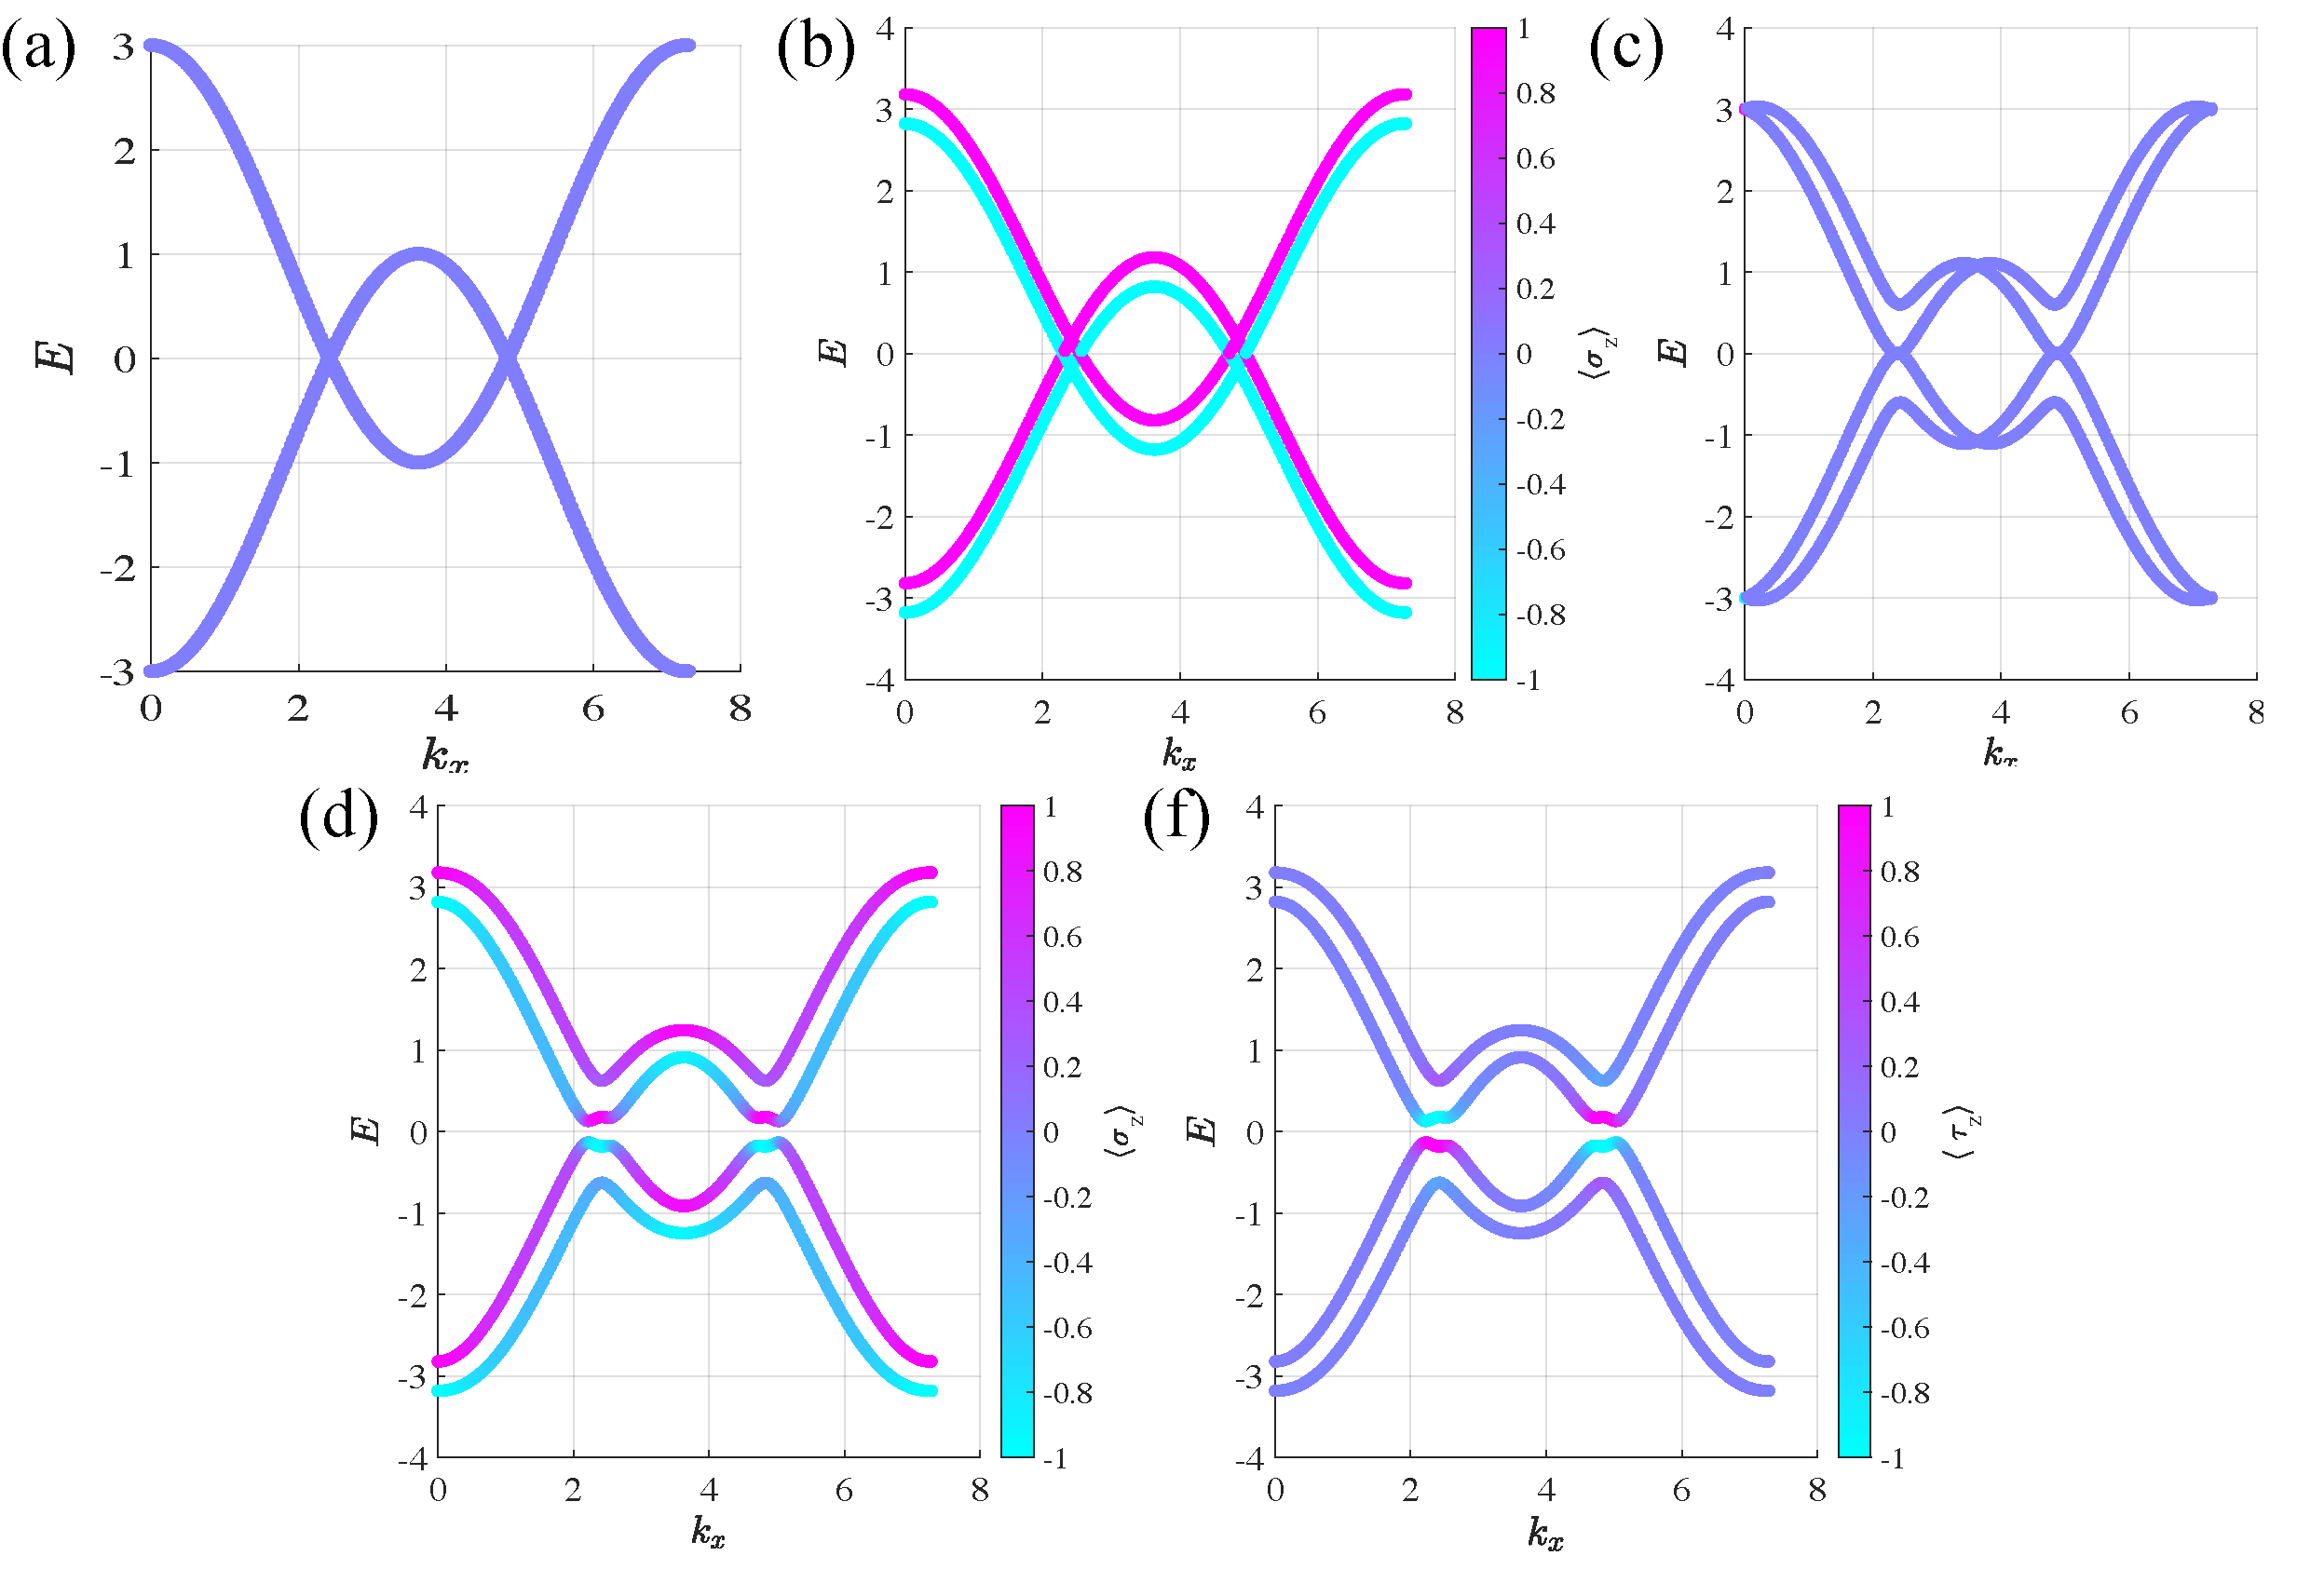
\includegraphics[width=0.5\textwidth]{pic/fig1.pdf}
	    \caption{(a)当$t_{\text{SO}}=0,\lambda=0,k_y=0$时的能带结构;(b)当$t_{\text{SO}}=0,\lambda=0.18,k_y=0$时,能带和自旋随着$k_x$变化;(c)当$t_{\text{SO}}=0.2,\lambda=0,k_y=0$时的能带结构;(d)能带和自旋随着$k_x$变化(f)能带和子晶格$\langle \tau_z\rangle$随着$ k_x$变化。(d-f)中的参数为$t_{\text{SO}}=0.2,\lambda=0.18,k_y=0$。}	    \label{fig1:BandStructure}
	\end{figure}
	
	
	由于拓扑材料的体边对应(bulk-edge correspondence)性质\cite{Hasan2010},能带的总体拓扑性质可以通过边缘态色散和波函数分布来判断。因此,我们分别采用了纳米带结构下的格点模型\cite{Qi2006}和迭代格林函数\cite{sancho1985}来研究Zigzag边缘态的性质。
	
	在纳米带下,石墨烯的晶体结构如图\ref{fig2:OPB}~(a),相对于无限大体系,Zigzag边界的纳米带元胞有4个子晶格(已用绿色方框标出)。由于x方向仍然具有平移对称性,所以,$k_x$仍然是好量子数,取y方向的两端开边界,求解出边缘态色散。

	半无限大块材通过自能会对表面能带和表面态密度造成影响,因此,我们利用迭代格林函数可以得到求得表面态密度。迭代格林函数的逻辑方法如下:1. 分别建立表面哈密顿量$H_S$和体部分的哈密顿量$H_R$,同时,根据总体对称性,我们可以把体部分当成一个个一维链,链与链之间的连接由$H_{R_i,R_{i+1}}$表示;2.由于x方向仍然具有平移不变性,各部分哈密顿量可以写为$k_x$的Bloch哈密顿量;3.根据Lopez提出的迭代格林函数快速收敛方法\cite{sancho1985},我们可以利用下式进行截断求解,得到表面格林函数。
	\begin{equation}
	    \left\{
	    \begin{aligned}
	    G_s&=(\epsilon-H_S-\sum _R)^{-1}  \\
	    \sum _R&=H_{S R_0} g_{R_0} H_{S,R_0}^\dagger\\
	    g_{R_0}&=(\epsilon-H_{R_0}-H_{R_0,R_1}T)^{-1}\\
        T&=t_0+\tilde{t}_0 t_1+\tilde{t}_0\tilde{t}_1t_2+...+\tilde{t}_0\tilde{t}_1\dots t_N
	    \end{aligned}
	    \right.
	\end{equation}
    \[
    \begin{aligned}
    t_0&=(\epsilon-H_{R_0})^{-1}H_{R_0,R_1}^\dagger\\
    \tilde{t}_0&=(\epsilon-H_{R_0})^{-1}H_{R_0,R_1}\\
    t_i&=(\mathbb{I}-t_{i-1}\tilde{t}_{i_1}-\tilde{t}_{i_1} t_{i-1})^{-1} t_{i-1}^2 \\
    \tilde{t}_i&=(\mathbb{I}-t_{i-1}\tilde{t}_{i_1}-\tilde{t}_{i_1} t_{i-1})^{-1} \tilde{t}_{i-1}^2
    \end{aligned}
    \]
    不难从上式看出,迭代格林函数方法假设了链与链之间只有最近邻的连接。半无限大体部分对于表面部分的影响是通过最近邻的链连接进入表面部分的自能中。表面格林函数可以这样得到:
    \begin{equation}
      N(\epsilon)=-\frac{1}{\pi}\text{Im}\sum_{\alpha} G_S^{\alpha,\alpha}(k_x,\epsilon+i\eta)
    \end{equation}


    \begin{figure}
      \centering
     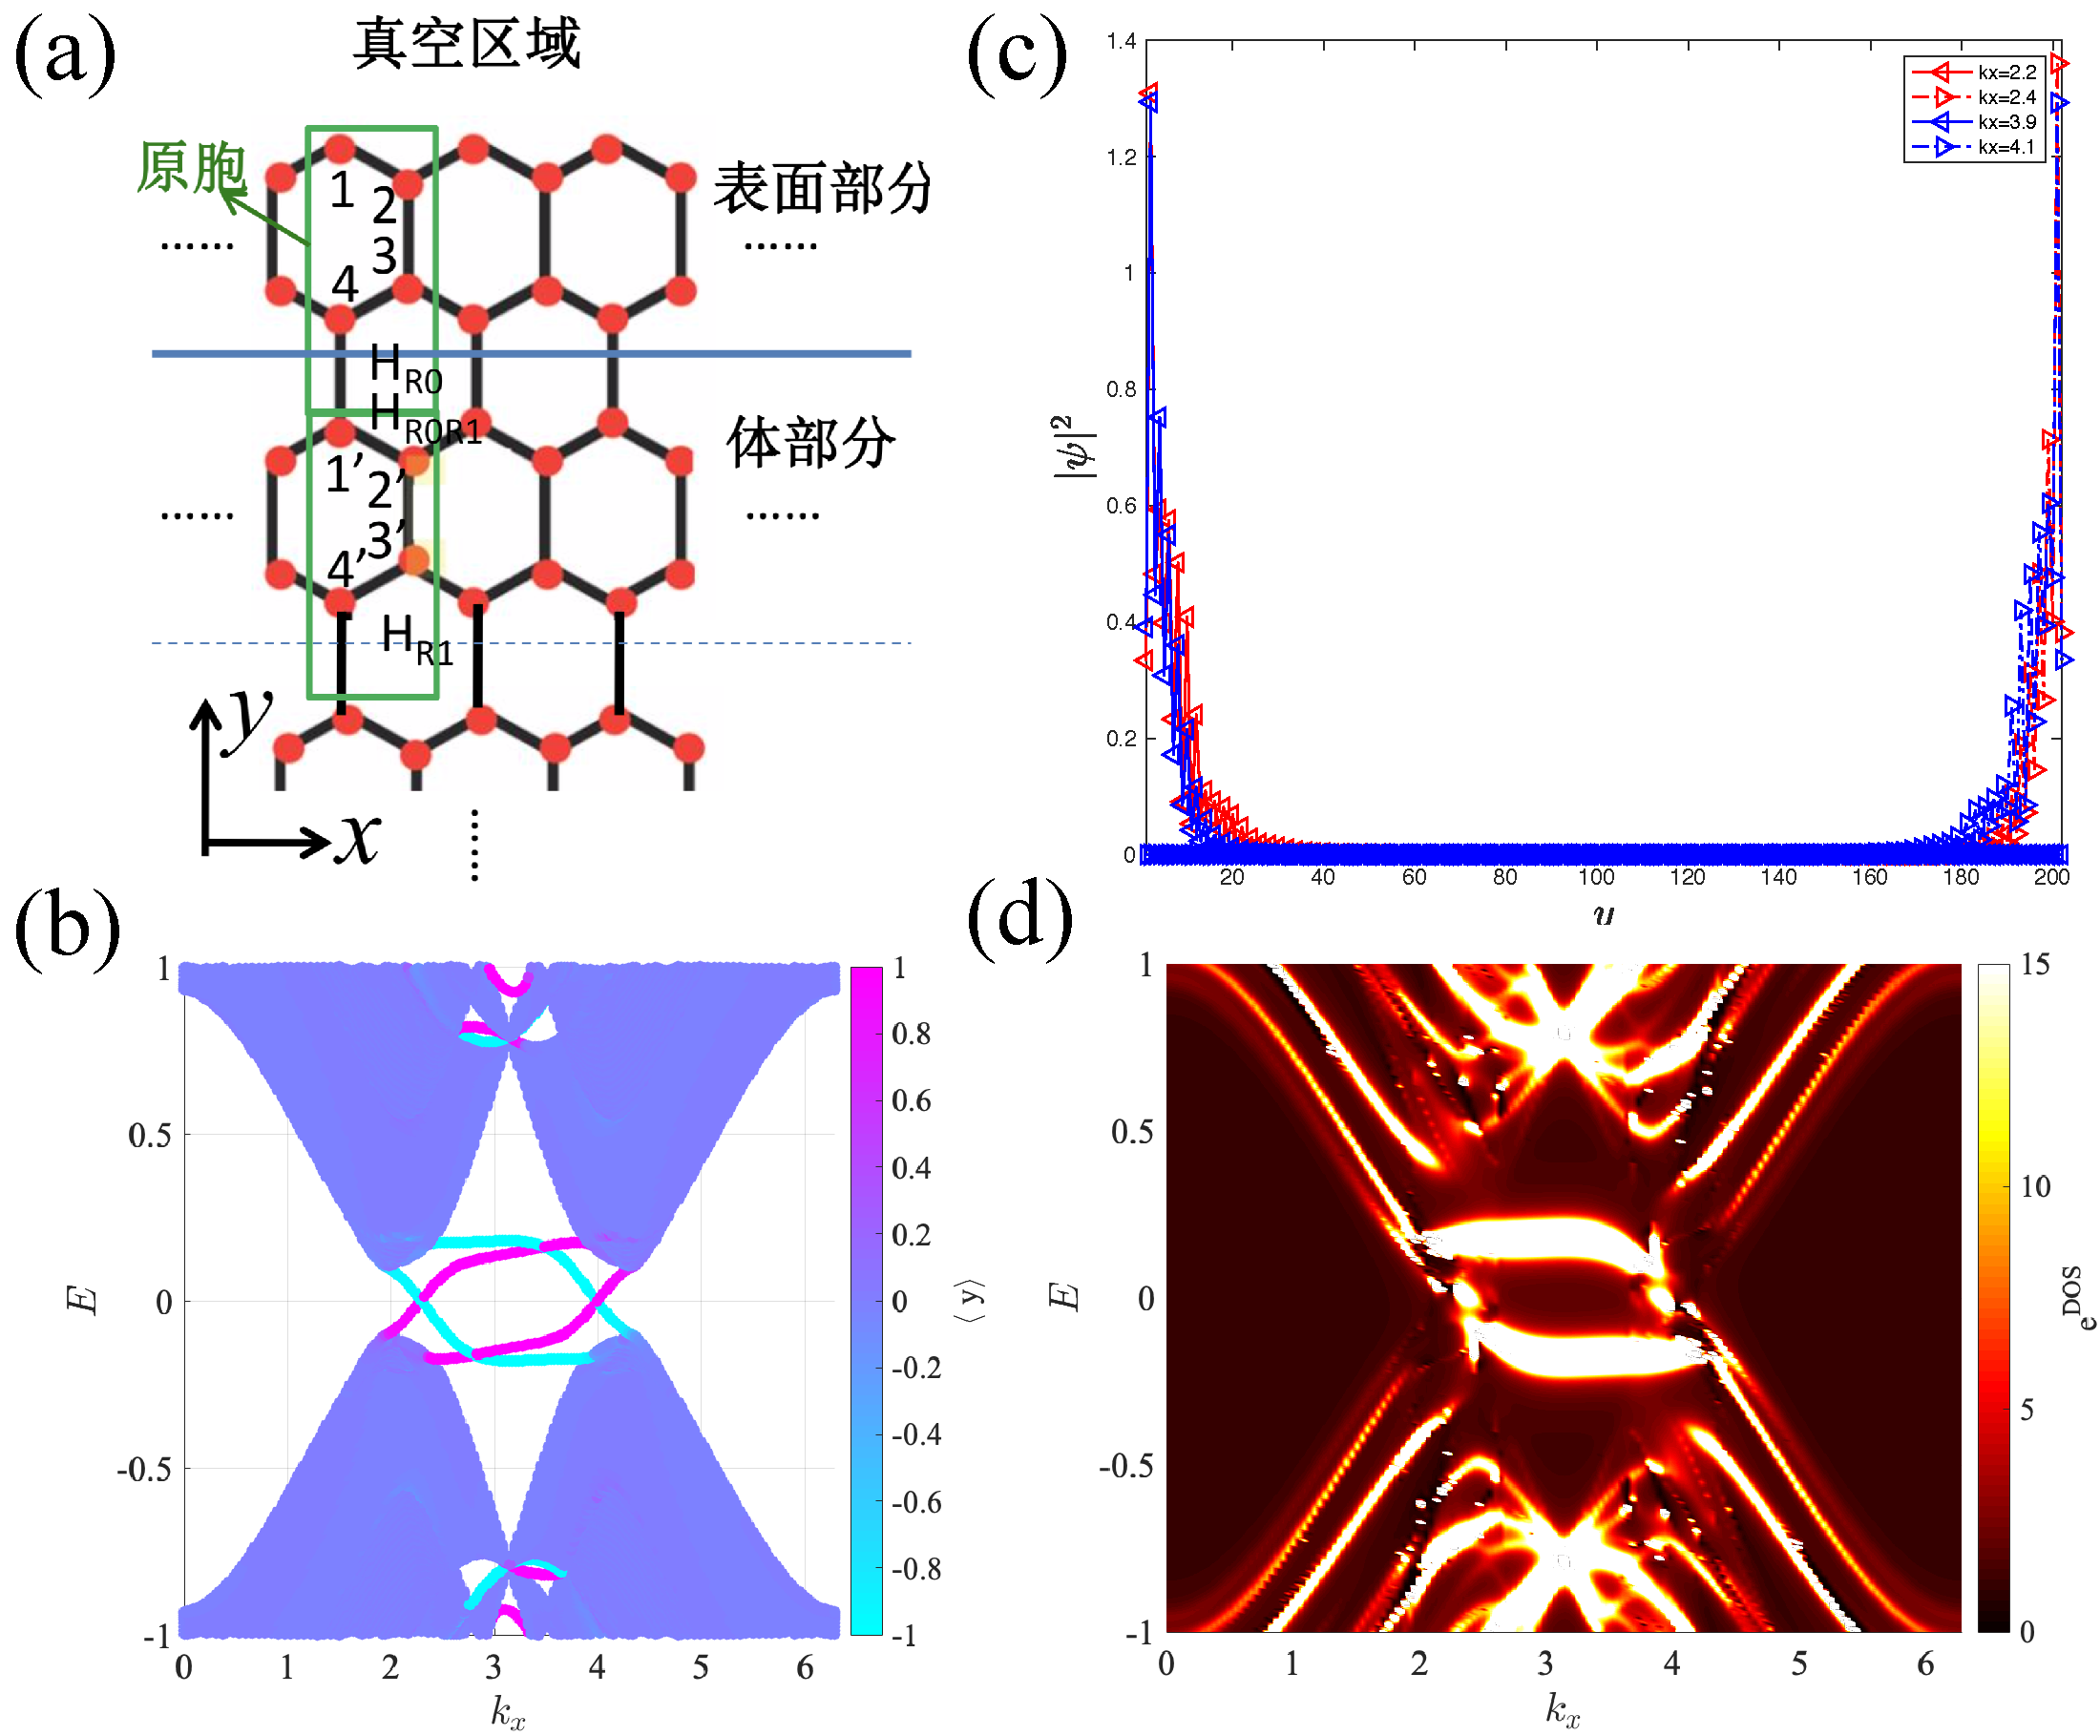
\includegraphics[width=0.5\textwidth]{pic/fig2.pdf}
      \caption{(a)纳米带结构下Zigzag开边界的石墨烯结构;(b)纳米带结构下格点模型的边缘态色散谱及其波函数的位置相对期望,从\ref{fig2:OPB}最上端至最下端,分别标为0,$L_y$;(c)纳米带结构下格点模型中$E_F=0.04t$时边缘态的波函数分布;(d)迭代格林函数得到的表面态密度(Surface DOS).参数分别为$t=1.0,t_{\text{SO}}=0.2,\lambda=0.18,L_y=200.$}
	    \label{fig2:OPB}
    \end{figure}

    \section{边缘态输运分析}\label{sec:result}
    现在,我们主要关注Zigzag边缘态的性质。图\ref{fig2:OPB}~(d)为用格林函数法解出的电子态密度(打开一侧$y$方向的zigzag链形成边界,将算得的态密度投影到$y_\text{min}=0$处),可清晰地看到一条明显区别于体态的无能隙手性边缘态:当费米面处于能隙中时,与边缘态色散有两个交点,且这两个电子态均沿着-$x$方向传播。

    为进一步理解所得边缘态与边界的关系,通过设置$y$方向为开边界,进行边缘态能谱和波函数计算。图\ref{fig2:OPB}~(b)表示了边缘态能谱,每个点对应的颜色表示波函数的位置期望,计为$\langle y\rangle=\frac{\langle \psi(k)\vert\hat{y} \vert \psi(k)\rangle-L_y/2}{Ly/2}$,其中$L_y$是$y$方向的格点数。两根蓝色(粉色)的线代表从$\mathbf{K}$($\mathbf{K}'$)到$\mathbf{K}'$($\mathbf{K}$)点的手性边缘态,对应在实空间中为同一个边界上的电子分别沿相同方向的运动,Chern
数应当为2。其中蓝色的边缘态的位置对应着图\ref{fig2:OPB}~(a)最上方的边界与图\ref{fig2:OPB}~(d)符合。当费米面为$0.04t$时,计算这四个边缘态上的电子波函数沿y方向石墨烯原胞数增加时的分布情况,观察到它极大地分布在两侧的原胞内,而在体态中间的原胞内基本为0,沿$-x$方向的电子($k_x=2.2,3.9$)集中在上表面,沿+x方向的电子($k_x=2.4,4.1$)集中在下边界。并且,波函数具有明显奇偶振荡的规律,上表面的边缘态偏向于占据A格子,下表面边缘态偏向于占据B格子。这些结果均体现出打开了石墨烯边界后沿Zigzag链上的手性边缘态特征。

    本征的无限大石墨烯体系因Dirac锥在$\mathbf{K}$、$\mathbf{K}'$点相交,自身属无带隙材料,而当同时考虑自旋轨道耦合与磁交换作用后,带隙在会在高对称点处打开。但在实验中,石墨烯样品总有边界,在边界上电子的单向传输正会对应到动量空间中连接$\mathbf{K}$与$\mathbf{K}'$点的手性边缘态,导致材料体态绝缘、边缘导电的输运性质。

    在实验上,石墨烯在输运性质上表现出非常奇特的特性。通过强磁场低温下的输运研究,研究者可以清晰的得出费米面在Dirac点附近时,电子的激发模式表现出无质量狄拉克费米子的特点,通过进一步研究,在磁场下,霍尔电阻出现一系列平台,同时出现磁阻在对应磁场为$0$的现象,这是典型的量子霍尔效应的特点。但是与以往量子霍尔效应不同的是,在石墨烯中霍尔电阻出现平台时的电阻值为1/2、3/2、5/2、7/2,对应的朗道能级分别是2、6、10、14,这意味着在石墨烯在磁场的作用下形成量子化的朗道能级,但是每个朗道能级是四重简并的,其中二重简并来源于上表面的能带,二重简并来源于下表面的能带,这正好和我们的理论计算相吻合,更为惊喜的是,在强磁场下,会出现1/2态,这正是手性边缘态的证据。当体系在强磁场的作用下进入量子极限之后,手性边缘态表现出第零级朗道能级,因此出现1/2,-1/2的态,分别对应手性不同的两个边缘态,这和理论计算完全吻合。


    \section{总结}\label{sec:summary}
    我们首先通过计算二维无限大的石墨烯能带结构,得到线性的Dirac锥结构和四重简并的Dirac点。由于,等价第一布里渊区存在两个等价Dirac锥,通过引入Rashba自旋轨道耦合和磁交换场作用,使得两个Dirac锥同时Band Inversion,实现了从拓扑半金属到$C=2$量子反常霍尔效应的转变。当考虑Zigzag链的半无限大平面时,通过迭代方法解出打开一侧Zigzag链边界后、半无限大石墨烯表面的格林函数,观察到在该能隙中出现了电子态密度的极值,这对应着连接其K到K’点之间的手性边缘传输态,同时有限格点模型得到的电子波函数空间分布也验证了这一点。虽然,实验上石墨烯的SOC强度较弱,难以实现有效调控。但是,本文给出了基于多Dirac锥体系实现高Chern数量子反常霍尔效应的思路,希望在之后的实验中得以实现。
 %这是正文

%----------------------------------------------------------------------------------------
%	REFERENCE LIST
%----------------------------------------------------------------------------------------

\phantomsection
\small
\renewcommand\refname{参考文献}
\bibliographystyle{unsrt}
\bibliography{essay/ref}

%\section{代码:Matlab}\label{sec:code}
\begin{lstlisting}[language=matlab]
%%%%%%%%%%%%%%%%%%%%%%%%%%%%%%%%%%%%%%%
% Band Structure
%%%%%%%%%%%%%%%%%%%%%%%%%%%%%%%%%%%%%%%

clear;
sigma_x=[0,1;1,0];sigma_y=1j*[0,-1;1,0];sigma_z=[1,0;0,-1];
% sigma_{ij}=tau_i sigma_j
sigma_x0=kron(sigma_x,eye(2));sigma_y0=kron(sigma_y,eye(2));
sigma_z0=kron(sigma_z,eye(2));
sigma_0x=kron(eye(2),sigma_x);sigma_0y=kron(eye(2),sigma_y);
sigma_0z=kron(eye(2),sigma_z);
sigma_zx=kron(sigma_z,sigma_x);sigma_zy=kron(sigma_z,sigma_y);
sigma_xx=kron(sigma_x,sigma_x);sigma_xy=kron(sigma_x,sigma_y);
sigma_yx=kron(sigma_y,sigma_x);sigma_yy=kron(sigma_y,sigma_y);
sigma_z0=kron(sigma_z,eye(2));sigma_zz=kron(sigma_z,sigma_z);
spin_operator=kron(eye(2),sigma_z);
orbit_operator=kron(sigma_z,eye(2));

kx_min=0;kx_max=2*pi;n_kx=211;
ky_min=-pi;ky_max=pi;n_ky=171;
kx_list=linspace(kx_min,kx_max,n_kx);
ky_list=linspace(ky_min,ky_max,n_ky);
Ham=zeros(4,4);
t=1;a=1;lambda=0.1;tso=0.2;V=0.;lambda_stagger=0.;
Ene=zeros(n_kx,n_ky,4);
Spin=zeros(n_kx,n_ky,4);
orbit=zeros(n_kx,n_ky,4);
for i_kx=1:n_kx
    kx=kx_list(i_kx);
    for i_ky=1:n_ky
        ky=ky_list(i_ky);
        Ham=-t*(2*cos(sqrt(3)/2*kx*a)*cos(ky/2*a)+cos(ky*a))*sigma_x0...
            -t*(-2*cos(sqrt(3)/2*kx*a)*sin(ky/2*a)+sin(ky*a))*sigma_y0...
            +lambda*sigma_0z...
            -tso*(cos(ky*a/2)*cos(sqrt(3)/2*kx*a)-cos(ky*a))*sigma_yx...
            -tso*sqrt(3)*sin(ky*a/2)*sin(sqrt(3)/2*kx*a)*sigma_yy...
            -tso*(sin(ky*a/2)*cos(sqrt(3)/2*kx*a)+sin(ky*a))*sigma_xx...
            -tso*sqrt(3)*(-cos(ky/2*a)*sin(sqrt(3)/2*kx*a))*sigma_xy+V*sigma_z0...
            +lambda_stagger*sigma_zz;
        [vec,ene_temp]=eig(Ham);
        Ene(i_kx,i_ky,:)=diag(ene_temp);
        Spin(i_kx,i_ky,:)=diag(vec'*spin_operator*vec);
        orbit(i_kx,i_ky,:)=diag(vec'*orbit_operator*vec);
    end
end
figure
for i_band=1:4
    mesh(kx_list,ky_list,Ene(:,:,i_band)');hold on;
end
colorbar;xlabel('k_x');ylabel('k_y');

figure
subplot(1,2,1)
Kx_list_temp=kron(ones(1,4),kx_list');
Kx_list=reshape(Kx_list_temp,1,numel(Kx_list_temp));
temp=Ene(:,floor(n_ky/2)+1,:);Ene_re=reshape(temp,numel(kx_list),4);
Ene_Re=reshape(Ene_re,1,numel(Ene_re));
temp=Spin(:,floor(n_ky/2)+1,:);Spin_re=reshape(temp,numel(kx_list),4);
Spin_Re=reshape(Spin_re,1,numel(Spin_re));
scatter(Kx_list,Ene_Re,[],Spin_Re,'filled');
c=colorbar;colormap('cool');
caxis([-1,1]);
c.Label.String='\langle\sigma_z\rangle';
set(c,'Fontsize',16,'Fontname', 'Times New Roman');
xlabel('$k_x$','Interpreter','latex','fontsize',21,'Fontname', 'Times New Roman');
ylabel('$E$','Interpreter','latex','fontsize',21,'Fontname', 'Times New Roman');
set(gca,'fontsize',18,'Fontname', 'Times New Roman');
grid on;
subplot(1,2,2)
temp=orbit(:,floor(n_ky/2)+1,:);orbit_re=reshape(temp,numel(kx_list),4);
orbit_Re=reshape(orbit_re,1,numel(orbit_re));
scatter(Kx_list,Ene_Re,[],orbit_Re,'filled');
c=colorbar;colormap('cool');c.Label.String='\langle \tau_z\rangle';
caxis([-1,1]);
set(c,'Fontsize',16,'Fontname', 'Times New Roman');
set(gca,'fontsize',18,'Fontname', 'Times New Roman');
xlabel('$k_x$','Interpreter','latex','fontsize',21,'Fontname', 'Times New Roman');
ylabel('$E$','Interpreter','latex','fontsize',21,'Fontname', 'Times New Roman');
grid on;
%
% % figure
% % temp=Ene(:,floor(n_ky/2)+1,:);
% % Ene_re=reshape(temp,numel(kx_list),4);
% % plot(kx_list,Ene_re,'b')
%
%
% %
% % figure
% % temp=Ene(floor(n_kx/2)+1,:,:);
% % Ene_re=reshape(temp,numel(ky_list),4);
% % plot(ky_list,Ene_re)


%%%%%%%%%%%%%%%%%%%%%%%%%%%%%%%%%%%%%%%
% EdgeSpectrum_lattice_Model_OPC
%%%%%%%%%%%%%%%%%%%%%%%%%%%%%%%%%%%%%%%

clear;
sigma_x=[0,1;1,0];sigma_y=1j*[0,-1;1,0];sigma_z=[1,0;0,-1];

sigma_zeeman=kron(eye(4),sigma_z);
stagger=diag([1,-1,1,-1],0);
sigma_zeeman_stagger=kron(stagger,sigma_z);
% spin_operator=kron(eye(2),sigma_z);
% orbit_operator=kron(sigma_z,eye(2));

kx_min=0;kx_max=2*pi;n_kx=201;
kx_list=linspace(kx_min,kx_max,n_kx);

t=1;a=1;lambda=0.18;tso=0.2;V=0.;lambda_stagger=0.;
Lx=a;sqrt(3)*a;
n_y=51;n_DOF=8;Ham=zeros(n_y*n_DOF,n_y*n_DOF);
Ene=zeros(n_kx,n_y*n_DOF);
position=zeros(n_kx,n_y*n_DOF);
sublattice=zeros(n_kx,n_y*n_DOF);

y_operator_temp=kron(linspace(-1,1,n_y),ones(1,8));
y_operator=diag(y_operator_temp,0);
sublattice_temp1=kron([1,-1,1,-1],ones(1,2));
sublattice_temp=kron(ones(1,n_y),sublattice_temp1);
sublattice_operator=diag(sublattice_temp,0);
for i_kx=1:n_kx
    kx=kx_list(i_kx);
%     same block
    temp=[1+exp(-1j*kx*Lx),1,1+exp(1j*kx*Lx)];
    h_hopping=diag(temp,1);
    h_hopping=h_hopping+h_hopping';
    H_hopping=kron(h_hopping,eye(2));
    temp=[-1j,0,0];xi_y_temp=diag(temp,1);xi_y_temp=xi_y_temp+xi_y_temp';
    temp=[1,0,0];xi_x_temp=diag(temp,1);xi_x_temp=xi_x_temp+xi_x_temp';
%     xi_{ij}=sigma_i xi_j
    xi_xy=kron(xi_y_temp,sigma_x);xi_yy=kron(xi_y_temp,sigma_y);
    xi_xx=kron(xi_x_temp,sigma_x);xi_yx=kron(xi_x_temp,sigma_y);
%     eta_{ij}=sigma_i eta_j
    temp=[0,0,-1j];eta_y_temp=diag(temp,1);eta_y_temp=eta_y_temp+eta_y_temp';
    temp=[0,0,1];eta_x_temp=diag(temp,1);eta_x_temp=eta_x_temp+eta_x_temp';
    eta_xy=kron(eta_y_temp,sigma_x);eta_yy=kron(eta_y_temp,sigma_y);
    eta_xx=kron(eta_x_temp,sigma_x);eta_yx=kron(eta_x_temp,sigma_y);
%     23 rashba
    temp=[0,-1j,0];matrix_23_temp=diag(temp,1);matrix_23_temp=matrix_23_temp+matrix_23_temp';
    matrix_23=kron(matrix_23_temp,sigma_x);
    matrix_potential=diag([1,1,-1,-1,1,1,-1,-1],0);
    for i_y=1:n_y
        Ham(n_DOF*(i_y-1)+1:n_DOF*(i_y),n_DOF*(i_y-1)+1:n_DOF*(i_y))=...
        -t*H_hopping+lambda*sigma_zeeman...
        +tso/2*(1+cos(kx*Lx))*xi_xy...
        -tso*sqrt(3)/2*(cos(kx*Lx)-1)*xi_yy...
        -tso/2*sin(kx*Lx)*xi_xx...
        +tso*sqrt(3)/2*sin(kx*Lx)*xi_yx...
        +tso/2*(1+cos(kx*Lx))*eta_xy...
        -tso*sqrt(3)/2*(cos(kx*Lx)+1)*eta_yy...
        +tso/2*sin(kx*Lx)*eta_xx...
        +tso*sqrt(3)/2*sin(kx*Lx)*eta_yx...
        +tso*matrix_23+V*matrix_potential+lambda_stagger*sigma_zeeman_stagger;
    end

%     different block
    h_hopping=diag([1],3);
    H_hopping=kron(h_hopping,eye(2));
    matrix_14_temp=diag([1j],3);
    matrix_14=kron(matrix_14_temp,sigma_x);
    i_y=1;
    Ham(n_DOF*(i_y-1)+1:n_DOF*(i_y),n_DOF*(i_y)+1:n_DOF*(i_y+1))=...
            -t*H_hopping+tso*matrix_14;
    for i_y=2:n_y-1
        Ham(n_DOF*(i_y-1)+1:n_DOF*(i_y),n_DOF*(i_y)+1:n_DOF*(i_y+1))=...
            -t*H_hopping+tso*matrix_14;
        Ham(n_DOF*(i_y-1)+1:n_DOF*(i_y),n_DOF*(i_y-2)+1:n_DOF*(i_y-1))=...
            Ham(n_DOF*(i_y-2)+1:n_DOF*(i_y-1),n_DOF*(i_y-1)+1:n_DOF*(i_y))';
    end
    i_y=n_y;
    Ham(n_DOF*(i_y-1)+1:n_DOF*(i_y),n_DOF*(i_y-2)+1:n_DOF*(i_y-1))=...
        Ham(n_DOF*(i_y-2)+1:n_DOF*(i_y-1),n_DOF*(i_y-1)+1:n_DOF*(i_y))';
    [vec,ene_temp]=eig(Ham);
    position(i_kx,:)=real(diag(vec'*y_operator*vec));
    sublattice(i_kx,:)=diag(vec'*sublattice_operator*vec);
    Ene(i_kx,:)=diag(ene_temp);
end
% figure
% plot(kx_list,Ene,'b');ylim([-1,1])

Kx_list_temp=kron(ones(1,n_y*n_DOF),kx_list');
Kx_list=reshape(Kx_list_temp,1,numel(Kx_list_temp));
Ene_scatter=reshape(Ene,1,numel(Ene));
position_scatter=reshape(position,1,numel(position));

sublattice_scatter=reshape(sublattice,1,numel(sublattice));

% figure
subplot(1,2,1)
scatter(Kx_list,Ene_scatter,[],position_scatter,'filled');colorbar;
c=colorbar;colormap('cool');c.Label.String='\langle y\rangle';
caxis([-1,1]);
xlim([kx_min,kx_max]);ylim([-1,1]);
set(c,'Fontsize',16,'Fontname', 'Times New Roman');
set(gca,'fontsize',18,'Fontname', 'Times New Roman');
xlabel('$k_x$','Interpreter','latex','fontsize',21,'Fontname', 'Times New Roman');
ylabel('$E$','Interpreter','latex','fontsize',21,'Fontname', 'Times New Roman');
grid on;hold off

subplot(1,2,2)
scatter(Kx_list,Ene_scatter,[],sublattice_scatter,'filled');colorbar;
c=colorbar;colormap('cool');c.Label.String='\langle \tau_z\rangle';
caxis([-1,1]);
xlim([kx_min,kx_max]);ylim([-1,1]);
set(c,'Fontsize',16,'Fontname', 'Times New Roman');
set(gca,'fontsize',18,'Fontname', 'Times New Roman');
xlabel('$k_x$','Interpreter','latex','fontsize',21,'Fontname', 'Times New Roman');
ylabel('$E$','Interpreter','latex','fontsize',21,'Fontname', 'Times New Roman');
grid on;hold off

%%%%%%%%%%%%%%%%%%%%%%%%%%%%%%%%%%%%%%%%%%%%%
% Wavefunction distribution_lattice_Model_OPC
%%%%%%%%%%%%%%%%%%%%%%%%%%%%%%%%%%%%%%%%%%%%%

clear;
sigma_x=[0,1;1,0];sigma_y=1j*[0,-1;1,0];sigma_z=[1,0;0,-1];

sigma_zeeman=kron(eye(4),sigma_z);
% spin_operator=kron(eye(2),sigma_z);
% orbit_operator=kron(sigma_z,eye(2));

kx_list=[2.2,2.4,3.9,4.1];n_kx=numel(kx_list);

t=1;a=1;lambda=0.18;tso=0.2;
Lx=a;
% sqrt(3)*a;
n_y=101;n_DOF=8;Ham=zeros(n_y*n_DOF,n_y*n_DOF);
Ene=zeros(n_kx,n_y*n_DOF);
position=zeros(n_kx,n_y*n_DOF);

y_operator_temp=kron(linspace(-1,1,n_y),ones(1,8));
y_operator=diag(y_operator_temp,0);
mat_temp=[1,1,0,0,1,1,0,0;0,0,1,1,0,0,1,1];
wav_pos_operator=kron(eye(n_y),mat_temp);
wav_pos=zeros(n_kx,n_y*2);
pos_list=linspace(1,n_y*2,n_y*2);

for i_kx=1:n_kx

    kx=kx_list(i_kx);
%     same block
    temp=[1+exp(-1j*kx*Lx),1,1+exp(1j*kx*Lx)];
    h_hopping=diag(temp,1);
    h_hopping=h_hopping+h_hopping';
    H_hopping=kron(h_hopping,eye(2));
    temp=[-1j,0,0];xi_y_temp=diag(temp,1);xi_y_temp=xi_y_temp+xi_y_temp';
    temp=[1,0,0];xi_x_temp=diag(temp,1);xi_x_temp=xi_x_temp+xi_x_temp';
%     xi_{ij}=sigma_i xi_j
    xi_xy=kron(xi_y_temp,sigma_x);xi_yy=kron(xi_y_temp,sigma_y);
    xi_xx=kron(xi_x_temp,sigma_x);xi_yx=kron(xi_x_temp,sigma_y);
%     eta_{ij}=sigma_i eta_j
    temp=[0,0,-1j];eta_y_temp=diag(temp,1);eta_y_temp=eta_y_temp+eta_y_temp';
    temp=[0,0,1];eta_x_temp=diag(temp,1);eta_x_temp=eta_x_temp+eta_x_temp';
    eta_xy=kron(eta_y_temp,sigma_x);eta_yy=kron(eta_y_temp,sigma_y);
    eta_xx=kron(eta_x_temp,sigma_x);eta_yx=kron(eta_x_temp,sigma_y);
%     23 rashba
    temp=[0,-1j,0];matrix_23_temp=diag(temp,1);matrix_23_temp=matrix_23_temp+matrix_23_temp';
    matrix_23=kron(matrix_23_temp,sigma_x);
    for i_y=1:n_y
        Ham(n_DOF*(i_y-1)+1:n_DOF*(i_y),n_DOF*(i_y-1)+1:n_DOF*(i_y))=...
        -t*H_hopping+lambda*sigma_zeeman...
        +tso/2*(1+cos(kx*Lx))*xi_xy...
        -tso*sqrt(3)/2*(cos(kx*Lx)-1)*xi_yy...
        -tso/2*sin(kx*Lx)*xi_xx...
        +tso*sqrt(3)/2*sin(kx*Lx)*xi_yx...
        +tso/2*(1+cos(kx*Lx))*eta_xy...
        -tso*sqrt(3)/2*(cos(kx*Lx)+1)*eta_yy...
        +tso/2*sin(kx*Lx)*eta_xx...
        +tso*sqrt(3)/2*sin(kx*Lx)*eta_yx...
        +tso*matrix_23;
    end

%     different block
    h_hopping=diag([1],3);
    H_hopping=kron(h_hopping,eye(2));
    matrix_14_temp=diag([1j],3);
    matrix_14=kron(matrix_14_temp,sigma_x);
    i_y=1;
    Ham(n_DOF*(i_y-1)+1:n_DOF*(i_y),n_DOF*(i_y)+1:n_DOF*(i_y+1))=...
            -t*H_hopping+tso*matrix_14;
    for i_y=2:n_y-1
        Ham(n_DOF*(i_y-1)+1:n_DOF*(i_y),n_DOF*(i_y)+1:n_DOF*(i_y+1))=...
            -t*H_hopping+tso*matrix_14;
        Ham(n_DOF*(i_y-1)+1:n_DOF*(i_y),n_DOF*(i_y-2)+1:n_DOF*(i_y-1))=...
            Ham(n_DOF*(i_y-2)+1:n_DOF*(i_y-1),n_DOF*(i_y-1)+1:n_DOF*(i_y))';
    end
    i_y=n_y;
    Ham(n_DOF*(i_y-1)+1:n_DOF*(i_y),n_DOF*(i_y-2)+1:n_DOF*(i_y-1))=...
        Ham(n_DOF*(i_y-2)+1:n_DOF*(i_y-1),n_DOF*(i_y-1)+1:n_DOF*(i_y))';
    [vec,ene_temp]=eig(Ham);
    wav=abs(vec(:,floor(n_y*n_DOF/2)+1));

    wav_pos(i_kx,:)=wav_pos_operator*wav;
    Ene(i_kx,:)=diag(ene_temp);

end
% figure
% plot(kx_list,Ene,'b');ylim([-1,1])

%r:K;b:K';<: negative velocity; >:positive velocity;
% figure
% plot(pos_list,wav_pos(1,:),'r<-','Linewidth',1,'MarkerSize',8);hold on;
% plot(pos_list,wav_pos(2,:),'r>-.','Linewidth',1,'MarkerSize',8);
% plot(pos_list,wav_pos(3,:),'b<-','Linewidth',1,'MarkerSize',8);
% plot(pos_list,wav_pos(4,:),'b>-.','Linewidth',1,'MarkerSize',8);
% xlim([1,n_y*2]);
% ylabel('$\vert \psi\vert^2$','Interpreter','latex','fontsize',21,'Fontname', 'Times New Roman');
% xlabel('$y$','Interpreter','latex','fontsize',21,'Fontname', 'Times New Roman');
% legend('kx=2.2','kx=2.4','kx=3.9','kx=4.1');
% hold off;

%%%%%%%%%%%%%%%%%%%%%%%%%%%%%%%%%%%%%%%
% Iterative Green Function
%%%%%%%%%%%%%%%%%%%%%%%%%%%%%%%%%%%%%%%

clear;
sigma_x=[0,1;1,0];sigma_y=1j*[0,-1;1,0];sigma_z=[1,0;0,-1];

sigma_zeeman=kron(eye(4),sigma_z);
% spin_operator=kron(eye(2),sigma_z);
% orbit_operator=kron(sigma_z,eye(2));

kx_min=0;kx_max=2*pi;n_kx=151;kx_list=linspace(kx_min,kx_max,n_kx);

t=1;a=1;lambda=0.18;tso=0.2;n_DOF=8;
E_min=-1.0;E_max=1.0;n_E=301;E_list=linspace(E_min,E_max,n_E);
E_imag_temp=0.3e-1;E_list=E_list+1j*E_imag_temp;
n_iter=10;

Lx=a;

DOS=zeros(n_kx,n_E);


for i_kx=1:n_kx
    kx=kx_list(i_kx);

    temp=[1+exp(-1j*kx*Lx),1,1+exp(1j*kx*Lx)];
    h_hopping=diag(temp,1);
    h_hopping=h_hopping+h_hopping';
    H_hopping=kron(h_hopping,eye(2));
    temp=[-1j,0,0];xi_y_temp=diag(temp,1);xi_y_temp=xi_y_temp+xi_y_temp';
    temp=[1,0,0];xi_x_temp=diag(temp,1);xi_x_temp=xi_x_temp+xi_x_temp';
%     xi_{ij}=sigma_i xi_j
    xi_xy=kron(xi_y_temp,sigma_x);xi_yy=kron(xi_y_temp,sigma_y);
    xi_xx=kron(xi_x_temp,sigma_x);xi_yx=kron(xi_x_temp,sigma_y);
%     eta_{ij}=sigma_i eta_j
    temp=[0,0,-1j];eta_y_temp=diag(temp,1);eta_y_temp=eta_y_temp+eta_y_temp';
    temp=[0,0,1];eta_x_temp=diag(temp,1);eta_x_temp=eta_x_temp+eta_x_temp';
    eta_xy=kron(eta_y_temp,sigma_x);eta_yy=kron(eta_y_temp,sigma_y);
    eta_xx=kron(eta_x_temp,sigma_x);eta_yx=kron(eta_x_temp,sigma_y);
%     23 rashba
    temp=[0,-1j,0];matrix_23_temp=diag(temp,1);matrix_23_temp=matrix_23_temp+matrix_23_temp';
    matrix_23=kron(matrix_23_temp,sigma_x);

    Ham_block=...
        -t*H_hopping+lambda*sigma_zeeman...
        +tso/2*(1+cos(kx*Lx))*xi_xy...
        -tso*sqrt(3)/2*(cos(kx*Lx)-1)*xi_yy...
        -tso/2*sin(kx*Lx)*xi_xx...
        +tso*sqrt(3)/2*sin(kx*Lx)*xi_yx...
        +tso/2*(1+cos(kx*Lx))*eta_xy...
        -tso*sqrt(3)/2*(cos(kx*Lx)+1)*eta_yy...
        +tso/2*sin(kx*Lx)*eta_xx...
        +tso*sqrt(3)/2*sin(kx*Lx)*eta_yx...
        +tso*matrix_23;
%  H_R0_R1  c_{j+1}^\dagger c_j
    h_hopping=diag([1],3);
    H_hopping=kron(h_hopping,eye(2));
    matrix_14_temp=diag([1j],3);
    matrix_14=kron(matrix_14_temp,sigma_x);

    Ham_linking=-t*H_hopping+tso*matrix_14;

    for i_E=1:n_E
        E_imag=E_list(i_E);
        t0=inv(E_imag*eye(8)-Ham_block)*Ham_linking';
        t0_tilted=inv(E_imag*eye(8)-Ham_block)*Ham_linking;
        ti=t0;ti_tilted=t0_tilted;
        T=ti;T_i=ti_tilted;
        for i_iter=1:n_iter
            t_temp=pinv(eye(8)-ti*ti_tilted-ti_tilted*ti)*ti*ti;
            t_temp_iter=pinv(eye(8)-ti*ti_tilted-ti_tilted*ti)*ti_tilted*ti_tilted;
            ti=t_temp;
            ti_iter=t_temp_iter;
            T=T+T_i*ti;
            T_i=T_i*ti_tilted;
        end
        g_R0=inv(E_imag*eye(8)-Ham_block-Ham_linking*T);
        sum_R=Ham_linking*g_R0*Ham_linking';
        G_S=inv(E_imag*eye(8)-Ham_block-sum_R);
        DOS(i_kx,i_E)=-1/pi*imag(sum(diag(G_S)));
    end
end
% figure
subplot(1,2,2)
surf(kx_list,real(E_list),exp(DOS'));shading('interp');
view(0,90);xlim([kx_min,kx_max]);ylim([E_min,E_max]);
c=colorbar;
caxis([0,15]);c.Label.String='e^{DOS}';
set(c,'Fontsize',16,'Fontname', 'Times New Roman');
set(gca,'fontsize',18,'Fontname', 'Times New Roman');
xlabel('$k_x$','Interpreter','latex','fontsize',21,'Fontname', 'Times New Roman');
ylabel('$E$','Interpreter','latex','fontsize',21,'Fontname', 'Times New Roman');
colormap('hot');
\end{lstlisting} 

%----------------------------------------------------------------------------------------

\end{document} 